\documentclass[12pt]{article}
\usepackage[T1]{fontenc}
\usepackage[polish]{babel}
\usepackage[utf8]{inputenc}
\usepackage{graphicx}
\usepackage{amsfonts}
\usepackage{amsmath}
\usepackage{float}
\usepackage{hyperref}

\newcommand{\BibTeX}{{\sc Bib}\TeX} 
\setlength{\textheight}{21cm}

\title{{\bf Zadanie nr 1 -- Generacja sygnału i szumu}\linebreak
Cyfrowe Przetwarzanie Sygnałów}

\author{Łukasz Murza, 251592 \and Aleksander Kaźmierczak, 251544}
\date{22 marca 2026}

\begin{document}

\maketitle
\thispagestyle{empty}
\newpage
\setcounter{page}{1}

\section{Cel zadania}
Celem ćwiczenia jest zapoznanie się z wybranymi własnościami podstawowych rodzajów sygnałów oraz implementacja aplikacji umożliwiającej ich generację, analizę statystyczną oraz wizualizację \cite{1}. Zadanie obejmuje stworzenie narzędzi do pracy z sygnałami ciągłymi (próbkowanymi) i dyskretnymi, a także wykonywanie podstawowych operacji arytmetycznych na ich amplitudach \cite{1}.

\section{Wstęp teoretyczny}
W ramach zadania zaimplementowano generator obsługujący 11 wariantów sygnałów i szumów, w tym szum o rozkładzie jednostajnym, szum gaussowski oraz sygnały okresowe, takie jak sinusoida czy sygnał prostokątny \cite{1}. 

Istotnym elementem analizy jest wyznaczanie parametrów statystycznych sygnału \cite{1}. Dla sygnałów dyskretnych (próbkowanych) zaimplementowano następujące wzory:
\begin{itemize}
    \item \textbf{Wartość średnia:} $\overline{x}=\frac{1}{n_{2}-n_{1}+1}\sum_{n=n_{1}}^{n_{2}}x(n)$ \cite{1}.
    \item \textbf{Wariancja:} $\sigma_{x}^{2}=\frac{1}{n_{2}-n_{1}+1}\sum_{n=n_{1}}^{n_{2}}[x(n)-\overline{x}]^{2}$ \cite{1}.
    \item \textbf{Wartość skuteczna (RMS):} $x_{RMS}=\sqrt{\frac{1}{n_{2}-n_{1}+1}\sum_{n=n_{1}}^{n_{2}}x^{2}(n)}$ \cite{1}.
\end{itemize}

W programie zaimplementowano dodatkowe parametry analizy energetycznej sygnału:
\begin{itemize}
    \item \textbf{Średnia wartość bezwzględna:} $|\overline{x}| = \frac{1}{n} \sum_{n=1}^{n} |x(n)|$.
    \item \textbf{Moc średnia:} $P_x = \frac{1}{n} \sum_{n=1}^{n} |x(n)|^2$.
\end{itemize}

W przypadku sygnałów okresowych, obliczenia są prowadzone dla całkowitej liczby okresów, z pominięciem niepełnych cykli w przyjętym zakresie czasu \cite{1}.

\section{Opis implementacji}
Aplikacja została zaimplementowana w języku \texttt{Python} z wykorzystaniem biblioteki \texttt{PySide6} do budowy interfejsu graficznego. Obliczenia numeryczne zrealizowano przy pomocy biblioteki \texttt{NumPy}, a wizualizację sygnałów i histogramów za pomocą \texttt{Matplotlib}. W celu zapewnienia stabilności działania aplikacji podczas operacji dzielenia (D4), w klasie \texttt{Signal} zastosowano mechanizm \texttt{np.errstate} z biblioteki \texttt{NumPy}. Pozwala on na kontrolowaną obsługę wyjątków zmiennoprzecinkowych, takich jak dzielenie przez zero (\textit{divide by zero}) oraz operacje na wartościach nieokreślonych (\textit{invalid}). Zrezygnowano również z dodawania małej wartości (epsilon) do mianownika na rzecz wiernego odwzorowania matematycznego charakteru operacji. W miejscach, gdzie wartości dzielnika dążą do zera, wynikowa amplituda dąży do nieskończoności. Błędy te są ignorowane programowo, co pozwala na wygenerowanie i analizę sygnału wynikowego bez przerywania pracy aplikacji.

\subsection{Format zapisu binarnego}
Zgodnie z wymaganiami, zaimplementowano własny format binarny zapisu sygnału dyskretnego. Plik składa się z 21-bajtowego nagłówka oraz ciągu próbek:
\begin{itemize}
    \item \textbf{Nagłówek (21 bajtów):}
    \begin{itemize}
        \item Czas początkowy $t_1$ (8 bajtów, \texttt{double}),
        \item Częstotliwość próbkowania $f$ (8 bajtów, \texttt{double}),
        \item Flaga sygnału zespolonego (1 bajt, \texttt{bool}),
        \item Liczba próbek (4 bajty, \texttt{int}).
    \end{itemize}
    \item \textbf{Dane:} Wartości amplitud zapisane jako liczby zmiennoprzecinkowe podwójnej precyzji (\texttt{float64}).
\end{itemize}

\subsection{Algorytm obliczeniowy dla sygnałów okresowych}
Podstawowym elementem jest klasa \texttt{Calculator} i jej metoda \texttt{get\_full\_periods\_data}, która automatycznie wykrywa czas trwania sygnału i przycina dane tak, aby obliczenia parametrów statystycznych (średnia, RMS, wariancja) odbywały się wyłącznie na pełnej liczbie okresów $T$. Zapobiega to błędom estymacji parametrów dla sygnałów o krótkim czasie trwania.

\section{Instrukcja obsługi aplikacji}
\begin{enumerate}
    \item \textbf{Generacja:} Należy wybrać typ sygnału z listy rozwijanej (np. Sygnał Sinusoidalny), uzupełnić parametry w formularzu i kliknąć przycisk \textit{Generuj}.
    \item \textbf{Analiza:} Po wygenerowaniu, w panelu \textit{Parametry Sygnału} automatycznie wyświetlą się obliczone wartości statystyczne.
    \item \textbf{Histogram:} Suwak w sekcji \textit{Ustawienia Histogramu} pozwala na płynną zmianę liczby przedziałów (od 5 do 20) \cite{1}.
    \item \textbf{Operacje:} Aplikacja posiada system historii. Aby wykonać operację (np. dodawanie), należy wybrać dwa wcześniej wygenerowane lub wczytane sygnały z list \textit{Sygnał 1} i \textit{Sygnał 2}, wybrać rodzaj działania i kliknąć \textit{Wykonaj operację}.
\end{enumerate}

\section{Eksperymenty i wyniki}
Aplikacja pozwala na generację sygnałów o zadanej amplitudzie ($A$), czasie początkowym ($t_1$) i czasie trwania ($d$) \cite{1}. Eksperymenty mają na celu sprawdznie działania napisanego programu, oraz wizualizację sygnałów po dokonanych operacjach.

\subsection{Założenia eksperymentu: Generacja sygnałów bazowych}
W celu przeprowadzenia operacji arytmetycznych wygenerowano dwa sygnały o identycznym czasie trwania i częstotliwości próbkowania, co jest warunkiem koniecznym do poprawnej realizacji działań na ich amplitudach \cite{1}.

Sygnał sinusoidalny (oznaczony w instrukcji jako S3) to fundamentalny sygnał okresowy, którego amplituda zmienia się w czasie zgodnie z funkcją trygonometryczną sinus \cite{1}. 

\begin{table}[H]
    \centering
    \vspace{0.2cm}
    \begin{tabular}{|l|c|}
        \hline
        \textbf{Parametr} & \textbf{Wartość} \\ \hline
        \multicolumn{2}{|c|}{\textit{Parametry wejściowe}} \\ \hline
        Amplituda ($A$) & 10.0 \\ \hline
        Czas początkowy ($t_1$) [s] & 0.0 \\ \hline
        Czas trwania ($d$) [s] & 2.0 \\ \hline
        Częstotliwość próbkowania ($f$) [Hz] & 1000.0 \\ \hline
        Częstotliwość sygnału [Hz] & 2.0 \\ \hline
        Przesunięcie fazowe [rad] & 0.0 \\ \hline
        \multicolumn{2}{|c|}{\textit{Wyniki obliczeń (statystyka)}} \\ \hline
        Wartość średnia & 0.0 \\ \hline
        Wartość średnia bezwzględna & 6.36 \\ \hline
        Wartość skuteczna (RMS) & 7.07 \\ \hline
        Wariancja & 50.0 \\ \hline
        Moc średnia & 50.0 \\ \hline
    \end{tabular}
    \caption{Parametry i wyniki analizy statystycznej sygnału sinusoidalnego (S3)}
    \label{tab:wyniki_sinus}
\end{table}

Jest on powszechnie wykorzystywany w cyfrowym przetwarzaniu sygnałów jako baza do analizy bardziej złożonych przebiegów. Zaimplementowany generator wykorzystuje bibliotekę \texttt{NumPy} do precyzyjnego wyznaczania wartości próbek dla zadanego kroku czasowego.

\begin{figure}[H]
    \centering
    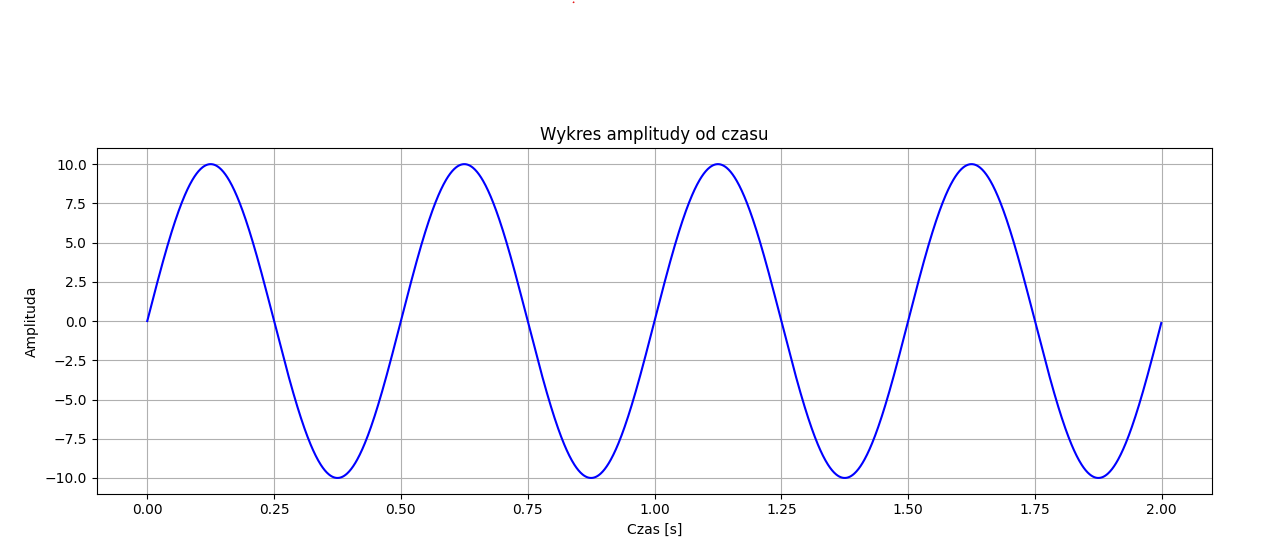
\includegraphics[width=0.85\linewidth]{sinus.png}
    \vspace{0.3cm} % Odstęp między obrazkami
    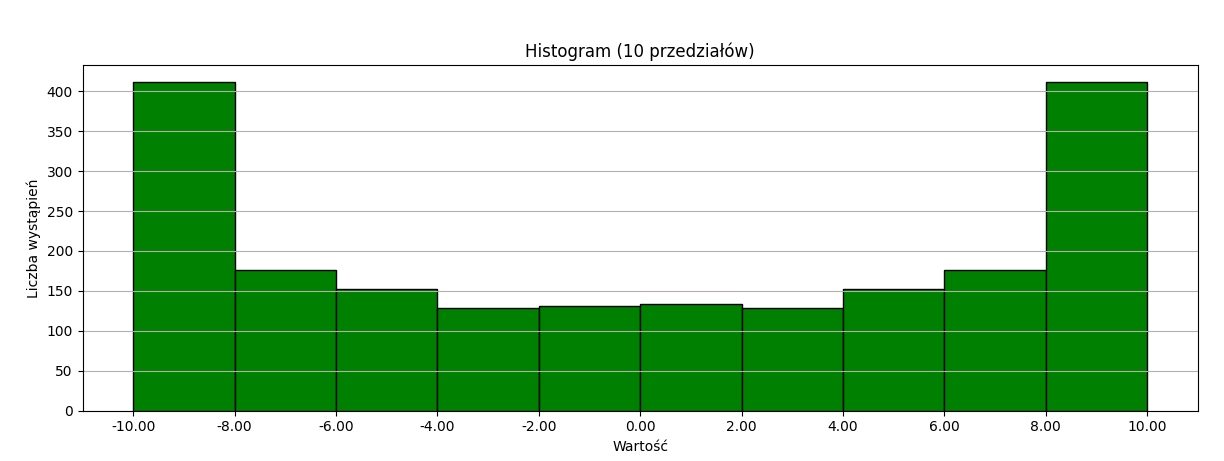
\includegraphics[width=0.85\linewidth]{sinus_histogram.png}
    \caption{Wizualizacja S3 sygnału sinusoidalnego: przebieg czasowy (góra) oraz odpowiadający mu histogram (dół).}
    \label{fig:sinus_wizualizacja}
\end{figure}

Szum gaussowski (oznaczony jako S2) to sygnał, w którym amplituda przyjmuje losowe wartości o rozkładzie normalnym (gaussowskim). 

\begin{table}[H]
    \centering
    \vspace{0.2cm}
    \begin{tabular}{|l|c|}
        \hline
        \textbf{Parametr / Wynik} & \textbf{Wartość} \\ \hline
        \multicolumn{2}{|c|}{\textit{Parametry wejściowe}} \\ \hline
        Amplituda ($A$) & 2.0 \\ \hline
        Czas początkowy ($t_1$) [s] & 0.0 \\ \hline
        Czas trwania ($d$) [s] & 2.0 \\ \hline
        Częstotliwość próbkowania ($f$) [Hz] & 1000.0 \\ \hline
        Średnia rozkładu ($\mu$) & 0.0 \\ \hline
        Odchylenie standardowe ($\sigma$) & 1.0 \\ \hline
        \multicolumn{2}{|c|}{\textit{Wyniki obliczeń (statystyka)}} \\ \hline
        Wartość średnia & 0.0242 \\ \hline
        Wartość średnia bezwzględna & 1.6182 \\ \hline
        Wartość skuteczna (RMS) & 2.0303 \\ \hline
        Wariancja & 4.1214 \\ \hline
        Moc średnia & 4.1220 \\ \hline
    \end{tabular}
    \caption{Parametry i wyniki analizy statystycznej szumu gaussowskiego (S2)}
    \label{tab:wyniki_szum_gauss}
\end{table}

Charakteryzuje się on tym, że większość próbek skupiona jest wokół wartości średniej, a prawdopodobieństwo wystąpienia wartości skrajnych gwałtownie spada zgodnie z funkcją gęstości rozkładu.

\begin{figure}[H]
    \centering
    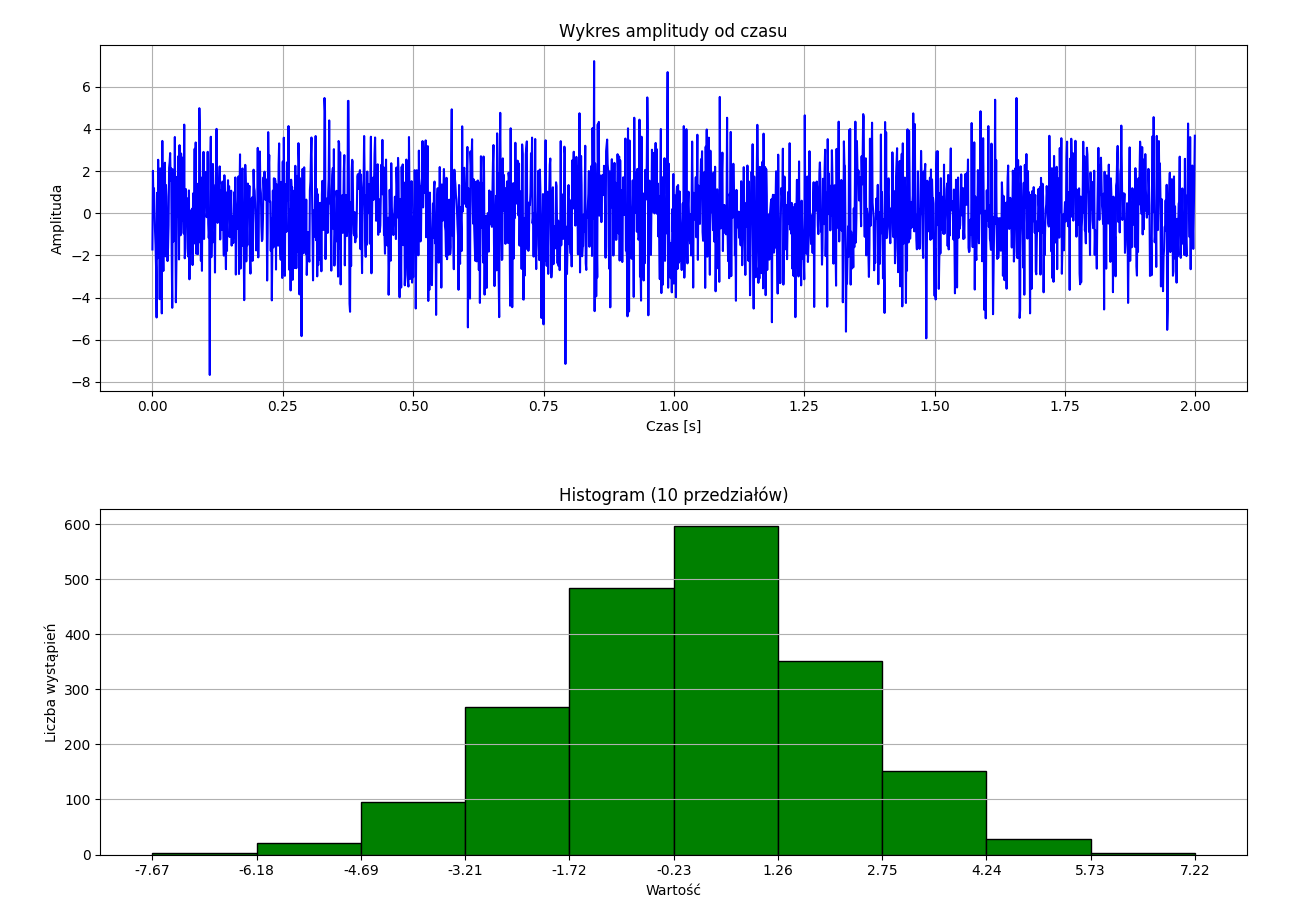
\includegraphics[width=0.85\linewidth]{szum_gausa.png}
    \caption{Wizualizacja szumu gaussowskiego S2: przebieg czasowy (góra) oraz odpowiadający mu histogram (dół).}
    \label{fig:szum_wizualizacja}
\end{figure}

\subsection{Eksperyment nr 2: Dodawanie sygnałów (D1)}
Przeprowadzono operację dodawania sygnału sinusoidalnego i szumu gaussowskiego \cite{1}. 

\begin{figure}[H]
    \centering
    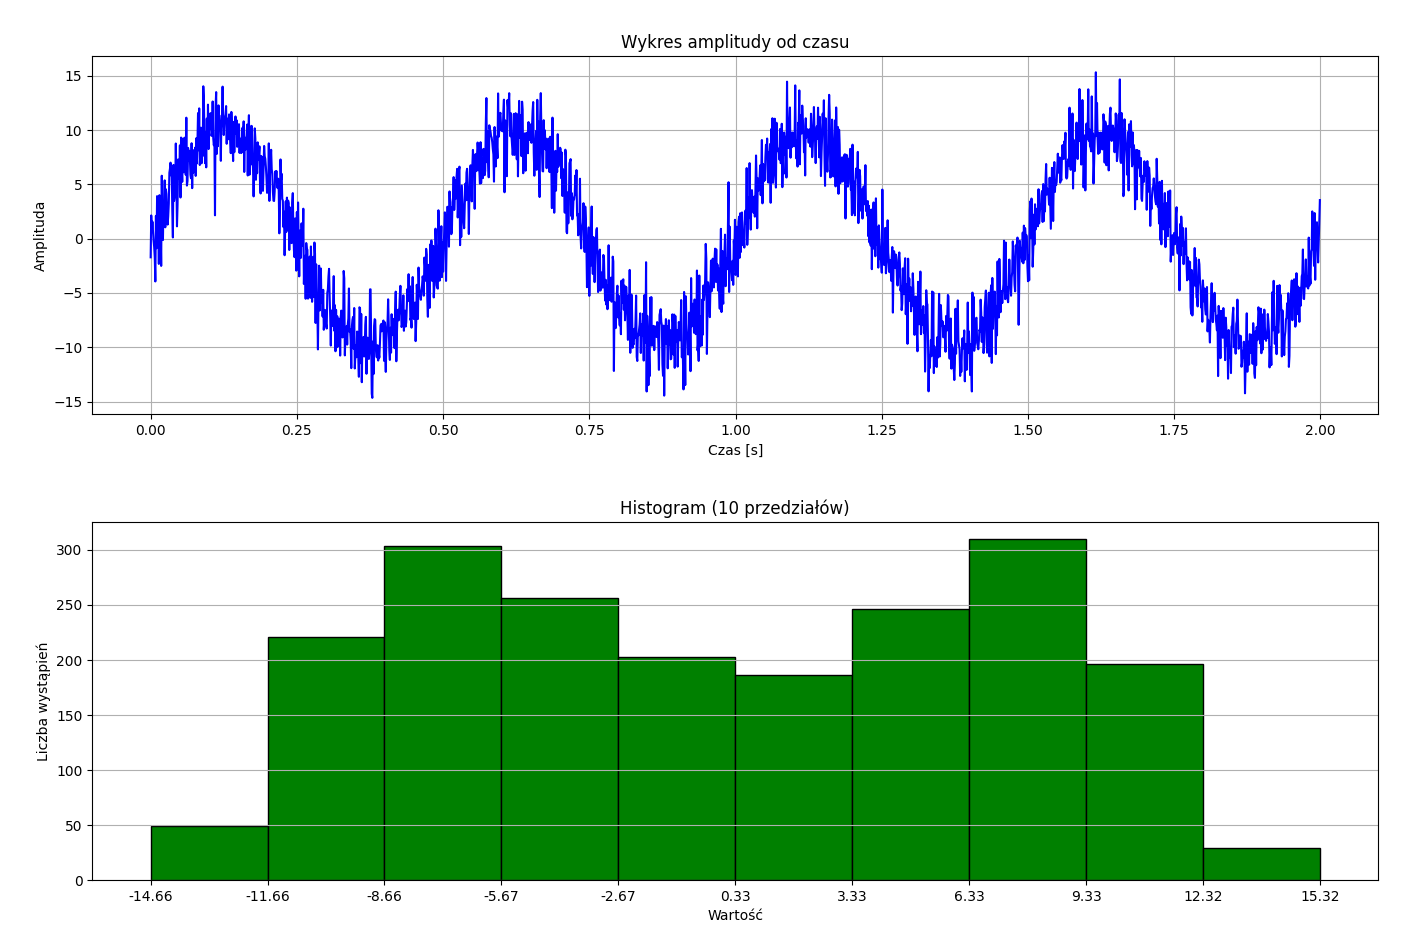
\includegraphics[width=0.85\linewidth]{dodanie.png}
    \caption{Wizualizacja dodania szumu gaussowskiego i sygnału sinusoidalnego: przebieg czasowy (góra) oraz odpowiadający mu histogram (dół).}
    \label{fig:dodanie_wizualizacja}
\end{figure}

\textbf{Rezultat:} Otrzymano sygnał sinusoidalny z widocznymi oscylacjami szumu wokół przebiegu głównego. Wartość średnia sygnału wynikowego jest zbliżona do sumy wartości średnich obu sygnałów składowych.

\subsection{Eksperyment nr 3: Odejmowanie sygnałów (D2)}
Od sygnału sinusoidalnego odjęto szum gaussowski \cite{1}.

\begin{figure}[H]
    \centering
    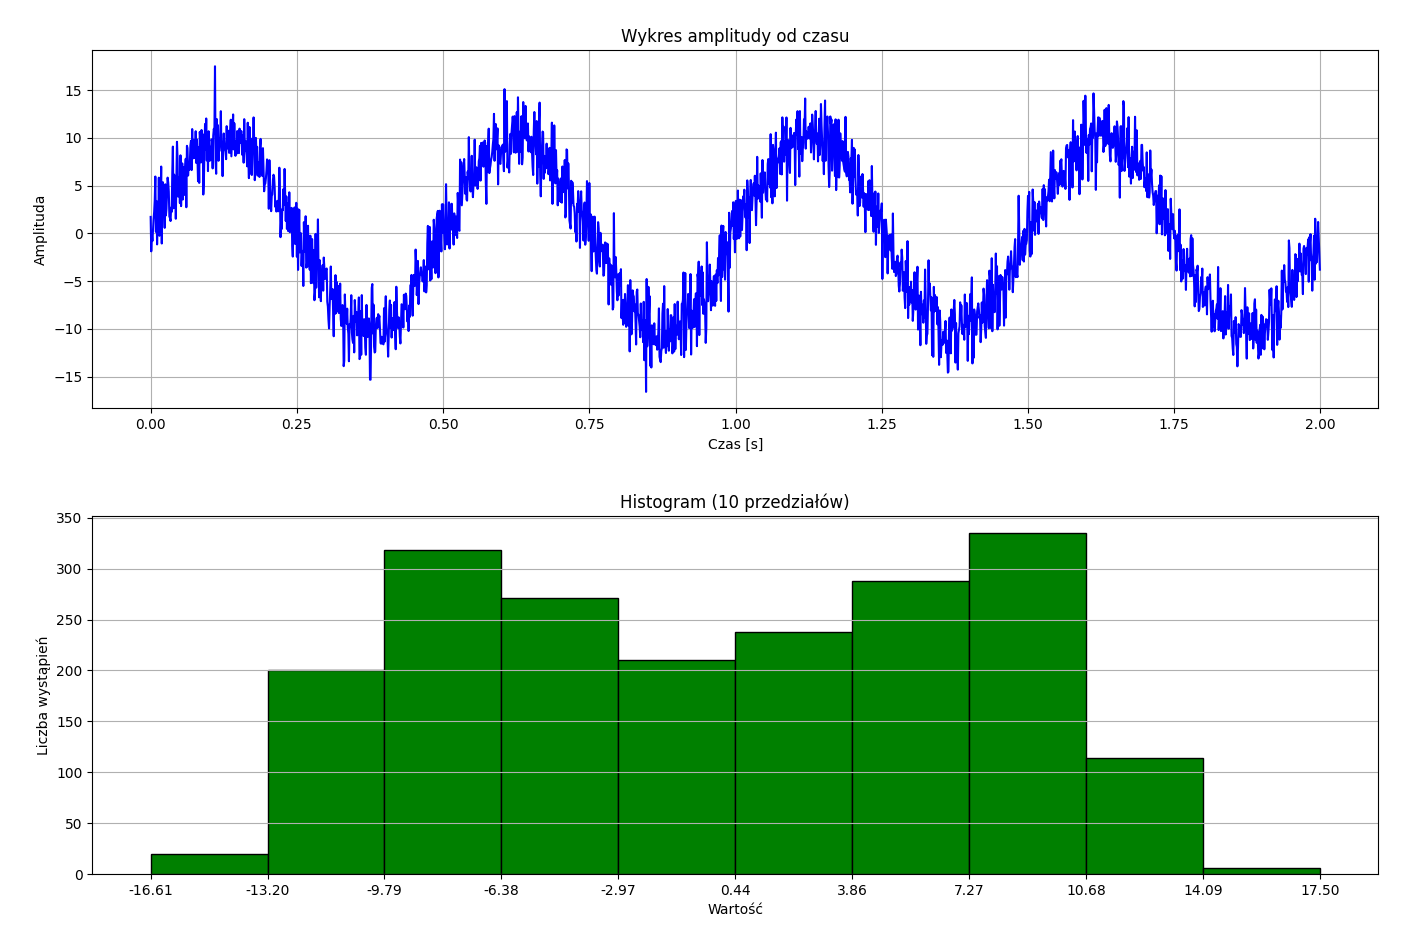
\includegraphics[width=0.85\linewidth]{odjecie.png}
    \caption{Wizualizacja odjęcia szumu gaussowskiego i sygnału sinusoidalnego: przebieg czasowy (góra) oraz odpowiadający mu histogram (dół).}
    \label{fig:odjecie_wizualizacja}
\end{figure}

\textbf{Rezultat:} Operacja ta, podobnie jak dodawanie, skutkuje zaszumieniem sinusoidy, jednak z odwróconą fazą składowej szumowej. Jest to proces fundamentalny przy testowaniu algorytmów odszumiania sygnałów.

\subsection{Eksperyment nr 4: Mnożenie sygnałów (D3)}
Wykonano mnożenie amplitudy sinusoidy przez wartości szumu gaussowskiego \cite{1}.

\begin{figure}[H]
    \centering
    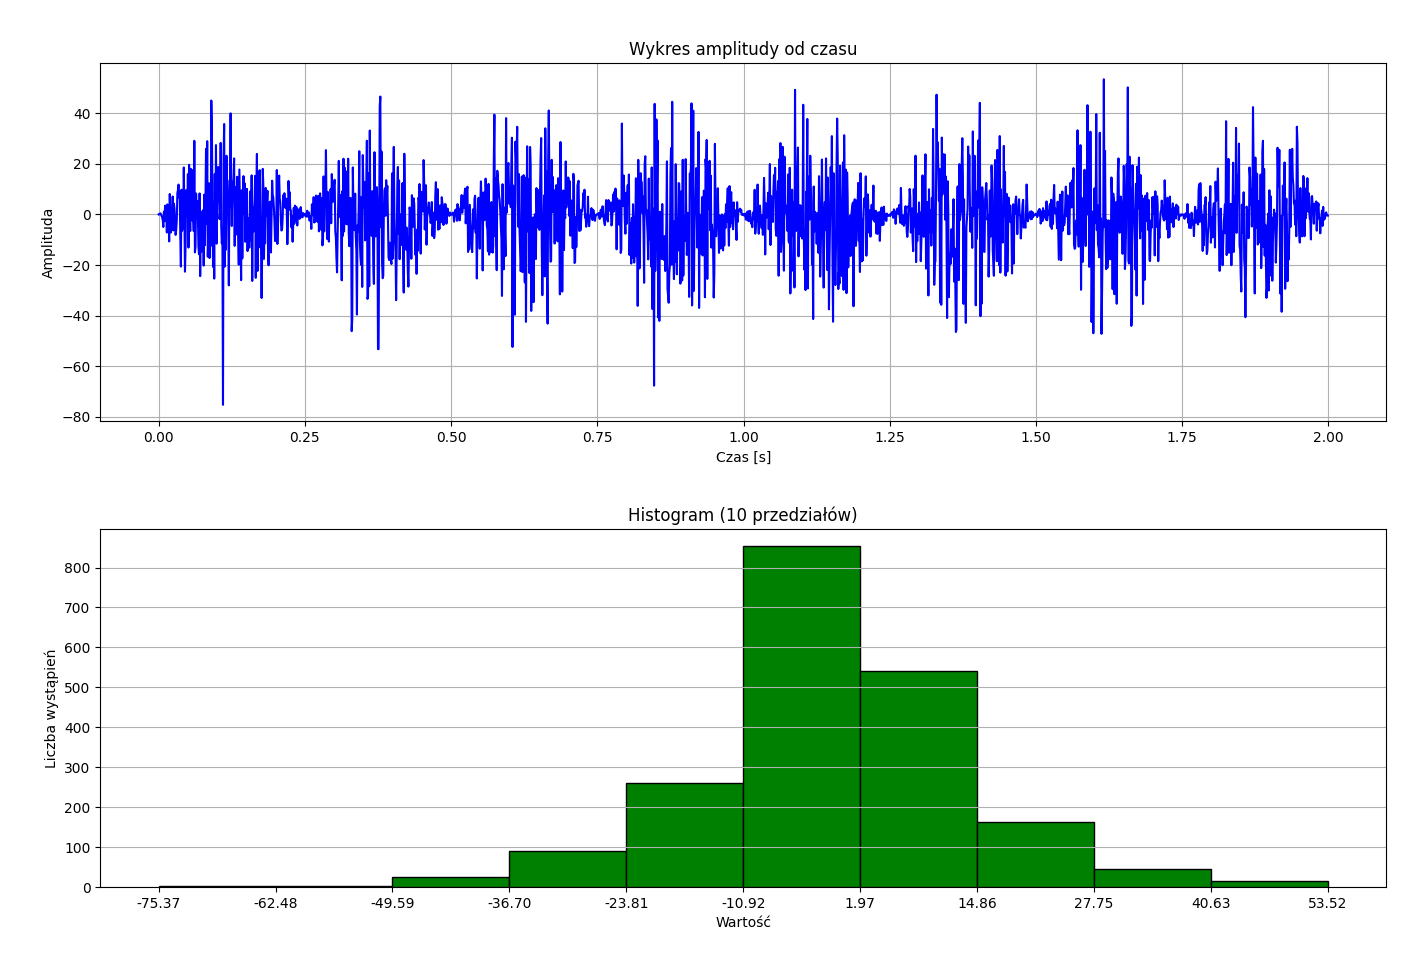
\includegraphics[width=0.85\linewidth]{mnozenie.png}
    \caption{Wizualizacja mnożenia szumu gaussowskiego i sygnału sinusoidalnego: przebieg czasowy (góra) oraz odpowiadający mu histogram (dół).}
    \label{fig:mnozenie_wizualizacja}
\end{figure}

\textbf{Rezultat:} Uzyskano efekt zbliżony do modulacji amplitudy (AM), gdzie szum pełni rolę sygnału modulującego. Amplituda sinusoidy "pulsuje" w rytm zmian losowych szumu, co znacząco zwiększa wariancję sygnału wynikowego.

\subsection{Eksperyment nr 5: Dzielenie sygnałów (D4)}
Podzielono wartości sygnału sinusoidalnego przez wartości szumu gaussowskiego \cite{1}.

\begin{figure}[H]
    \centering
    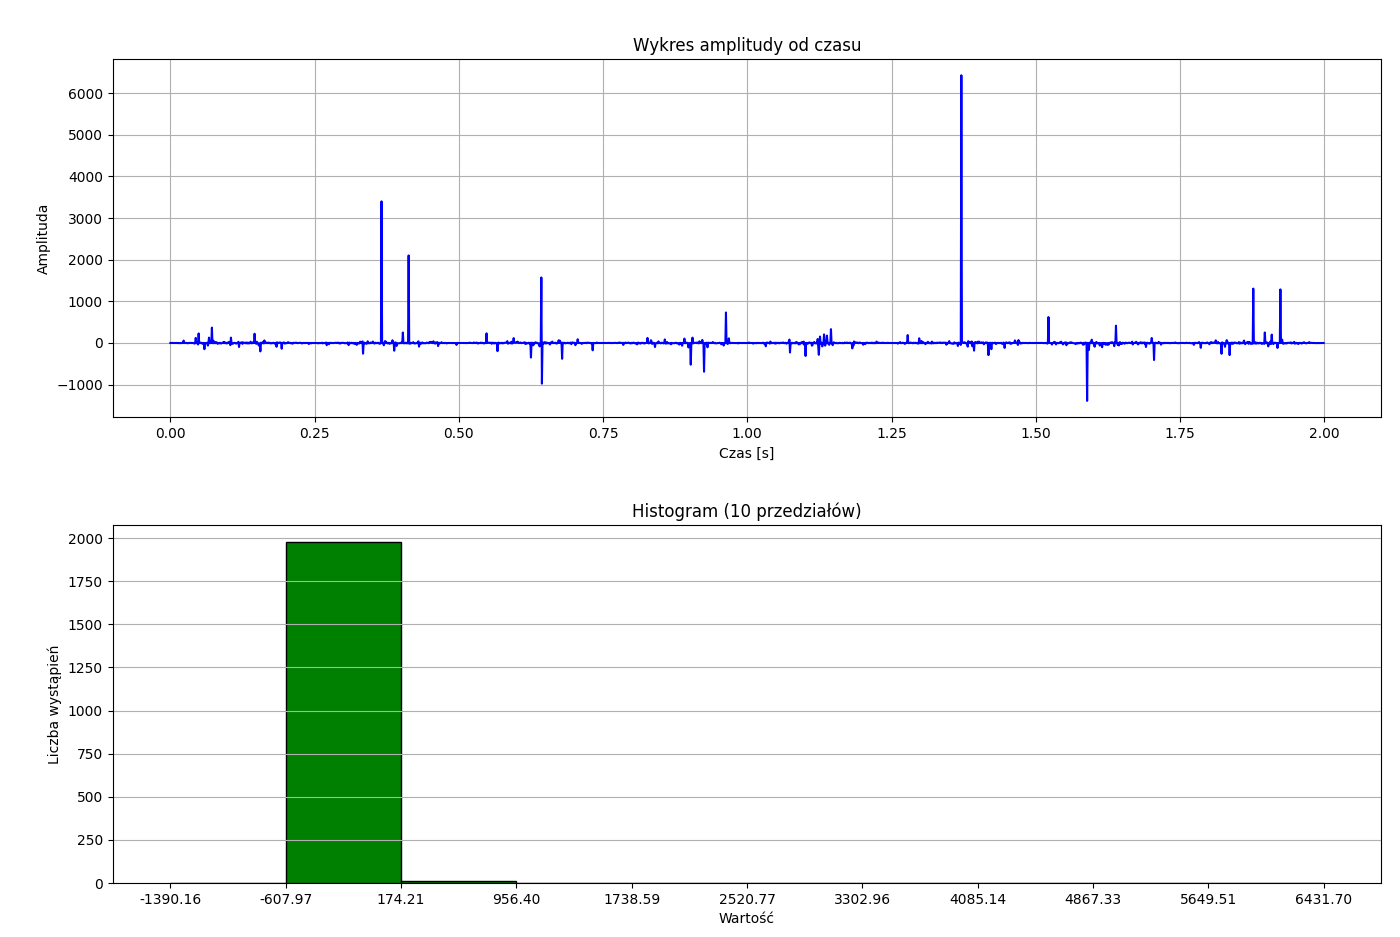
\includegraphics[width=0.85\linewidth]{dzielenie.png}
    \caption{Wizualizacja dzielenia szumu gaussowskiego i sygnału sinusoidalnego: przebieg czasowy (góra) oraz odpowiadający mu histogram (dół).}
    \label{fig:dzielenie_wizualizacja}
\end{figure}

\textbf{Rezultat:} Jest to najbardziej niestabilna operacja. W punktach, gdzie wartości szumu (dzielnika) są bliskie zeru, pojawiają się gwałtowne piki (szpilki) o bardzo wysokich amplitudach. Sygnał wynikowy charakteryzuje się ekstremalnie dużą mocą średnią i wariancją, co utrudnia jego klasyczną analizę statystyczną.

\subsection{Zbiorcze wyniki wszystkich przeprowadzonych eksperymentów}

\begin{table}[H]
    \centering
    \vspace{0.2cm}
    \begin{tabular}{l c c c}
        \hline\hline\\[-0.4cm]
        \textbf{Operacja} & \textbf{Wartość średnia} & \textbf{Wariancja} & \textbf{Wartość skut.} \\[0.1cm]
        \hline
        S1: Sinus    & 0.00  & 50.00 & 7.07 \\
        S2: Szum     & 0.02  & 4.12  & 2.03 \\
        \hline
        \textbf{D1: Dodawanie}   & 0.02  & 52.45 & 7.24 \\
        \textbf{D2: Odejmowanie} & -0.02 & 55.80 & 7.47 \\
        \textbf{D3: Mnożenie}    & -0.84 & 208.33 & 14.46 \\
        \textbf{D4: Dzielenie}   & 5.69  & 35279.57 & 187.91 \\ [0.1cm]
        \hline
    \end{tabular}
    \caption{Statystki po operacjach (D1--D4) – wartości zaokrąglone}
    \label{tab:wyniki_operacji_zaokraglone}
\end{table}

\section{Wnioski}
Implementacja algorytmów obliczeniowych potwierdziła, że parametry takie jak wartość skuteczna i moc średnia są niezbędne dla energetycznej oceny sygnału \cite{1}. Zastosowanie wymogu obliczeń dla pełnych okresów sygnałów periodycznych znacząco redukuje błędy estymacji wartości średniej i wariancji. Aplikacja poprawnie obsługuje eksport danych do formatu binarnego, co pozwala na dalszą obróbkę sygnałów w kolejnych etapach laboratorium \cite{1}.


\begin{thebibliography}{1}
\bibitem{1} Instrukcja do zadania 1: Generacja sygnału i szumu.
\end{thebibliography}

\end{document}